\section{Spørgsmål 7}

% Structured Query Language SQL, herunder begreberne DML og DDL, samt strukturen for og mulighederne med de forskellige typer SQL erklæringer.

\subsection{Fokuspunkter}
\begin{itemize}
	\item Structured Query Language SQL.
	\begin{itemize}
		\item Herunder begreberne DML og DDL.
		\item Samt strukturen for og mulighederne med de forskellige typer SQL erklæringer
	\end{itemize}
\end{itemize}

\subsection{Litteratur}
\begin{itemize}
	
	\item Fra teori: Database Modeling and Design. Logical Design 5'th Ed.
	\begin{itemize}
		\item Appendix "The Basics of SQL" page 261-277.
	\end{itemize}
	
	\item Fra Database eLearning: \url{http://db.grussell.org/index.html}.
	\begin{itemize}
		\item Ch. 3 SQL
		\begin{itemize}
			\item Simple SELECT statements.
			\item Logical Operators and Aggregation.
			\item JOINs and VIEWs.
			\item Subqueries and Schema.
			\item Order of Evaluation.
		\end{itemize}
	\end{itemize}
	
%	\item Fra wikipedia:
%	\begin{itemize}
%		\item 
%	\end{itemize}
%	
%	\item Fra Agile Data Home Page:
%	\begin{itemize}
%		\item 
%	\end{itemize}
\end{itemize}

\newpage

% must
\subsection{Structured Query Language SQL}
SQL er er special purpose sprog der bruges til at manage relationelle databaser.

SQL består af 3 moduler.

\textbf{DML - Data Manipulation Language}
\textbf{DDS - Data Definition Language}
\textbf{Data Control Language}

\subsubsection{Elementer i sproget}

\begin{itemize}
	\item Clauses: UPDATE, SET, WHERE osv.
	\item Expressions: X+1.
	\item Statements: X = X+1.
	\item Predicates: X = 'Y'
	\item Operators: Minder meget om standar C operatorer. Afvigelser og specielle SQL operatorer har vi følgende:
	\begin{itemize}
		\item $!=$ er i SQL $<>$
		\item BETWEEN - Eksempel \textbf{Cost BETWEEN X AND Y}
		\item LIKE - Match af nogen dele af en parameter. Eksempel \textbf{Name LIKE 'Hans'}
		\item IN - Lig med en eller flere parametre. Eksempel \textbf{Number IN (1,6,5)}
		\item IS eller IS NOT - Eksempel \textbf{Name IS NOT NULL}
		\item IS NOT DISTINCT FROM - dunno.
		\item AS - Ændre et fieldname ved visning. Eksempel \textbf{SELECT Name AS 'Navn'}
		\item AND OR NOT - logiske operatorer.
	\end{itemize}
	\item Statement terminator ;
	
\end{itemize}

\begin{figure}
\centering
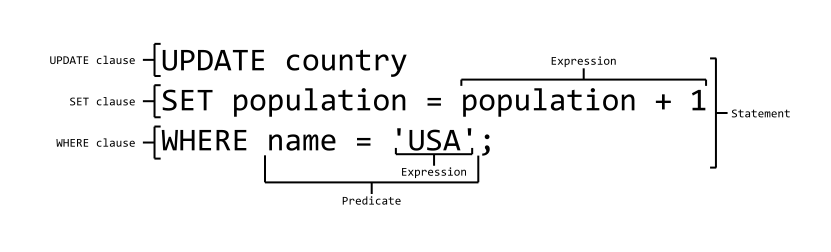
\includegraphics[width=0.9\linewidth]{figs/spm7/sqlDecomp}
\caption{Elemter i SQL}
\label{fig:sqlDecomp}
\end{figure}

% must
\subsubsection{Herunder begreberne DML og DDL}

\paragraph{DDL}
Bruges til at definere opbygning af databasens tabeller, relationer samt typedefinitioner på tabellernes attributter. Når man definerer en database bruges CREATE clausen.

\textbf{CREATE TABLE [table name] ( [column definitions] ) [table parameters]}

\begin{lstlisting}[caption=eksempel på CREATE]
CREATE TABLE [Blogs] (
[BlogId] INT            IDENTITY (1, 1) NOT NULL,
[Name]   NVARCHAR (MAX) NULL,
[Url]    NVARCHAR (MAX) NULL,
CONSTRAINT [PK_Blogs] PRIMARY KEY CLUSTERED ([BlogId] ASC)
);
\end{lstlisting}

\begin{itemize}
	\item IDENTITY (1,1) - Gør at DBMS selv imkrementerer Id'et med 1.
	\item NULL og NOT NULL - Specificerer om det er tilladt for attributten at være NULL.
	\item CONSTRAINT \textit{table\_name} PRIMARY KEY \textit{attr} - Specificerer at attributten er en primærnøgle.
\end{itemize}

\textbf{DROP TABLE [table name]}

DROP TABEL sletter en given tabel.\\

\textbf{TRUNCATE TABLE [table name]}

TRUNCATE TABLE sletter alt data i en given tabel.\\

\textbf{ALTER TABLE [table name] ADD [coloumn name] [type]}

\textbf{ALTER TABLE [table name] DROP COLOUMN [coloumn name] [type]}

ALTER TABLE ændrer i strukturen på en given tabel.\\

\textbf{RENAME TABLE [old\_name] TO [new\_name]}

RENAME TABLE ændrer tabellens navn.

\paragraph{DML}
DML er en syntaks samling der gør det muligt at manipulere data i en database.
DML bruges når vi vil arbejde med den data som allerede eksisterer i databasen, herunder lave Queries, Sub-queries, Insertions, Opdateringer, Sletninger og Merges.

\begin{itemize}
	\item \textbf{Queries} - Her anvendes SELECT. Se statement~\ref{select}. I dette statement bruges aggregate funktionen AVG som tager gennemsnittet. Af aggregate funktioner kan der bla nævnes: AVG, SUM, MAX, MIN og COUNT.
	\begin{lstlisting}[caption=Query med sub-query,label=select]
	SELECT pris, kalorier
	FROM  Varer
	WHERE pris < (SELECT AVG(pris) FROM Varer)
	ORDER BY pris;
	\end{lstlisting}
	
	I forbindelse med queries, kan der bruges JOIN, som gør det muligt udføre en multi-table query. Se eksempel~\ref{join med og uden JOIN}
	
	\begin{lstlisting}
	SELECT * 
	FROM mad, kage 
	WHERE navn = 'x'
	
	SELECT * 
	FROM mad 
	JOIN kage ON (navn='x') 
	\end{lstlisting}
		
	\item \textbf{Insertions} - Her anvendes INSERT. Se statement~\ref{insert}
	
	\begin{lstlisting}[caption=Brug af INSERT,label=insert]
	INSERT INTO Varer
	(pris, navn, kalorier)
	VALUES
	(10, 'Vand', 0);
	\end{lstlisting}
	
	\item \textbf{Opdateringer} - Her anvendes UPDATE. Se statement~\ref{update}
	
	\begin{lstlisting}[caption=Brug af UPDATE,label=update]
	UPDATE Varer
	SET pris = 5
	WHERE navn = 'Vand';
	\end{lstlisting}
	
	\item \textbf{Sletninger} - Her anvendes DELETE. Se statement~\ref{delete}
	
	\begin{lstlisting}[caption=brug af DELETE,label=delete]
	DELETE FROM Varer
	WHERE Navn = 'Vand';
	\end{lstlisting}
	
	\item \textbf{Merges} - Her anvendes MERGE. Se statement~\ref{merge}
	
	\begin{lstlisting}[caption=Brug af MERGE,label=merge]
	MERGE INTO table_name USING table_reference ON (condition)
	WHEN MATCHED THEN
	UPDATE SET column1 = value1 [, column2 = value2 ...]
	WHEN NOT MATCHED THEN
	INSERT (column1 [, column2 ...]) VALUES (value1 [, value2 ...])
	\end{lstlisting}
\end{itemize}
